\documentclass[a4paper]{article} 

%中文环境设置
\usepackage{xeCJK} 
\usepackage{indentfirst}
\setlength{\parindent}{2em}
\usepackage{enumitem}

\usepackage{abstract}
\renewcommand{\abstractname}{摘要}
\providecommand{\keywords}[1]{\textbf{\textit{关键词}} #1}

\setCJKmainfont{STSong} % 中文主字体设置 

\usepackage[colorlinks,linkcolor=blue, citecolor=blue]{hyperref}

% 常用宏包
\usepackage{float}
\usepackage{stfloats}
\usepackage{graphicx}
\usepackage{color}
\usepackage{supertabular}

% 代码环境设置
\usepackage{listings}
\lstset{
	columns=fullflexible,
 	frame=single,
 	breaklines=true,
}
\definecolor{lightgray}{gray}{0.9}
\newcommand{\inlinecode}[2]{\colorbox{lightgray}{\lstinline[language=#1]$#2$}}

% 页面段落设置
\usepackage{multicol}
\usepackage{geometry}
\geometry{left=3.18cm, right=3.18cm, top=2.54cm, bottom=2.54cm}
\linespread{1.3}
%\setlength{\parskip}{0.5em} 

% 数学环境设置
\usepackage{amsmath}
\usepackage{amssymb}
\usepackage{amsthm}
\usepackage{amsfonts}
\usepackage{mathrsfs}
\newtheorem{myDef}{Definition} 
\newtheorem{myThm}{Theorem}
\newtheorem{myProp}{Property}

\begin{document} 
\title{数值积分与数值微分\ 实验题}
\author{吴佳龙 2018013418}
\date{}
\maketitle

\begin{abstract}
	结合理论分析和编程计算,运用不同方法计算了一函数的数值积分。运用的方法分别为:五点 Gauss-Legendre 求积公式的复合求积公式和 Romberg 求积方法。
\end{abstract}

%\keywords{one, two, three, four}

\begin{multicols}{2}

\begin{section}{问题}

	用不同的数值积分方法计算 $$I(f)=\int_{1}^{3} f(x) d x=\int_{1}^{3} \frac{1}{x^{2}} \sin \frac{2 \pi}{x} d x$$ 准确解为:$I(f)=-0.238732414637843 \cdots$
	
	\begin{enumerate}
  		\item 把 $[1,3]$ 分成 $4$ 个子区间,用五点 Gauss-Legendre 求积公式的复合求积公式计算。
  		\item 用 Romberg 求积方法计算积分,取 $\varepsilon = 10^{-7}$,并与第一种办法比较。
	\end{enumerate}	

\end{section}

\begin{section}{五点 Gauss-Legendre 求积公式的复合求积公式}
	
	\begin{subsection}{算法原理}
		
		\begin{subsubsection}{Gauss 求积公式}
		
			Newton-Cotes 求积公式 $$\int_{a}^{b} f(x) \mathrm{d} x=(b-a) \sum_{i=1}^{n} c_{i k}^{(n)} f\left(x_{i}^{(n)}\right)+E_{n}(f)$$ 取等距的求积节点 $x_k^{(n)}$。对于 $n+1$ 个等距节点的插值型求积公式,其代数精度至多为 $n+1$。
			
			考虑适当选取 $n+1$ 个节点的位置,使得代数精度从 $n $ 或 $n+1$ 增加到 $2n+1$。
			
			Newton-Cotes 求积公式中余项为 $$E(f)=\frac{1}{(n+1) !} \int_{a}^{b} \rho(x) f^{(n+1)}(\xi(x)) \omega_{n+1}(x) \mathrm{d} x$$ 若要对 $f \in \mathscr{P}_{2 n+1}\Rightarrow f^{(n+1)} \in \mathscr{P}_{n}$ 都有 $E(f)=0$,可取 $\omega_{n+1}(x)$ 为 $[a,b]$ 上的 $n+1$ 次正交多项式,即取插值节点为 $[a,b]$ 上 $n+1$ 次正交多项式的零点。
			
			有以下定理:
			
			\begin{myThm}
				
				插值型求积公式具有 $2n+1$ 次代数精度的充分必要条件是求积节点是 $[a,b]$ 上权函数为 $\rho$ 的 $n+1$ 次正交多项式的零点。

			\end{myThm}

			
			该求积公式称为 Gauss 求积公式,相应的求积节点为Gauss 点。
			
			与 Newton-Cotes 公式不同,Gauss 求积公式的求积系数都是正数,从而 Gauss 求积是数值稳定的。另外,还可证明,Gauss 求积公式有收敛性: $$\lim _{n \rightarrow \infty} \sum_{k=0}^{n} A_{k}^{(n)} f\left(x_{k}^{(n)}\right) =\int_{a}^{b} \rho(x) f(x) \mathrm{d} x $$
			
		\end{subsubsection}
		
		\begin{subsubsection}{Gauss-Legendre 求积公式}
		
			在区间 $[-1,1]$ 上取权函数 $\rho(x) = 1$ 对应的 Gauss 求积公式称为 Gauss-Legendre 求积公式。
			
			其误差为
			
			$$E_{n}(f)=\frac{2^{2 n+3}[(n+1) !]^{4}}{(2 n+3)[(2 n+2) !]^{3}} f^{(2 n+2)}(\eta)$$
			
			取 $n=4$,五点 Gauss-Legendre 求积公式的 Gauss点和求积系数如下:
			
			\begin{table}[H]
			\centering
			\begin{tabular}{c|c}
			\hline
			\multicolumn{1}{c|}{$x_k$} & \multicolumn{1}{c}{$A_k$}        
			\\ \hline
			-0.9061798459 & 0.2369268851 \\
			-0.5384693101 & 0.4786286705 \\
			0 & 0.5688888889 \\
			0.5384693101 & 0.4786286705 \\
			0.9061798459 & 0.2369268851 \\ 
			\hline
			\end{tabular}
			\end{table}
			
			对一般区间 $[a,b]$,将其变换到 $[-1,1]$,有
			
			$$\int_{a}^{b} f(x) \mathrm{d} x=\frac{b-a}{2} \int_{-1}^{1} f\left[\frac{a+b}{2}+\frac{b-a}{2} t\right] \mathrm{d} t$$
			
		\end{subsubsection}
		
		\begin{subsubsection}{复合求积公式}
		
			为提高定积分的精度,将整个积分区间分成若干子区间,然后分别采用低阶求积公式。这种积分方法称为复合求积公式。
			
		\end{subsubsection}
		
	\end{subsection}

	\begin{subsection}{算法实现}
		
		五点 Gauss-Legendre 求积公式的 MATLAB 实现如下:
		
\begin{lstlisting}[language=Matlab]
function I = myGaussLegendre(f,a,b)
% 五点 Gauss-Legendre 求积公式求 f 在 [a,b] 上积分
xk = [-0.9061798459, -0.5384693101, 0, 0.5384693101, 0.9061798459];
Ak = [0.2369268851, 0.4786286705, 0.5688888889, 0.4786286705, 0.2369268851];
I = (b-a)/2*sum(f((a+b)/2+(b-a)/2*xk).*Ak);
end
\end{lstlisting}

		复合的五点 Gauss-Legendre 求积公式的 MATLAB 实现如下:
		
\begin{lstlisting}[language=Matlab]
function I = myCompositeGaussLegendre(f,a,b,n)
% 五点 Gauss-Legendre 求积公式复合求 f 在 [a,b] 上积分
% 将 [a,b] 等分成 n 段
I = 0;
for i=0:n-1
    ai = a+(b-a)/n*i;
    bi = a+(b-a)/n*(i+1);
    I = I + myGaussLegendre(f,ai,bi);
end
end
\end{lstlisting}

		
	\end{subsection}
	
	\begin{subsection}{计算结果}
	
		调用函数 \inlinecode{Matlab}{myCompositeGaussLegendre(@f,1,3,4)},得到数值解为 $$I(f)\approx -0.238732340355842$$
		
	\end{subsection}
	
\end{section}

\begin{section}{Romberg 求积方法}

	\begin{subsection}{算法原理}
		
		\begin{subsubsection}{Euler-Maclaurin 公式}
			
			令 $B_k$ 为 Bernoulli 数,有Euler-Maclaurin 求和公式 
			
			\begin{align}
				\nonumber
				&\int_{a}^{b} f(x) \mathrm{d} x-T_{n}(f) = \\
				\nonumber
				&-\sum_{i=1}^{m} \frac{B_{2 l}}{(2 l) !}\left[f^{(2 l-1)}(b)-f^{(2 l-1)}(a)\right] h^{2 l}+r_{m+1}
			\end{align}
			
			其中 $T_n(f)$ 为复合梯形求积公式,$r_{m+1}$ 为余项。
			
		\end{subsubsection}
		
		\begin{subsubsection}{Richardason 外推方法}
			
			用 $(T_1f)(h)$ 来表示 $T_n(f)$,由 Euler-Maclaurin 公式 $$I(f)-(T_1f)(h) = \alpha_2h^2 + O(h^4)$$ 将 $h$ 缩小一半,有 $$I(f)-(T_1f)({h\over 2}) = \alpha_2({h\over 2})^2+O(h^4)$$ 令 $$\left(T_{2} f\right)(h)=\frac{4\left(T_{1} f\right)\left(\frac{h}{2}\right)-\left(T_{1} f\right)(h)}{3}$$ 则 $$I(f)-(T_2f)(h) = O(h^4)$$ 将误差从 $O(h^2)$ 提高到了 $O(h^4)$。
			
			这种方法称为 Richardason 外推方法,详细描述与证明见课本。
			
		\end{subsubsection}

		\begin{subsubsection}{Romberg 求积方法}
			
			将 Euler-Maclaurin 公式 和 Richardason 外推方法结合,在外推算法中取 $q={1\over 2}, p_k = 2k$,得到 Romberg 求积方法。
			
			\begin{align}
				\nonumber
				\left(T_{1} f\right)(h)&=\frac{h}{2} \sum_{m=1}^{n}\left[f\left(x_{m-1}\right)+f\left(x_{m}\right)\right] \\
				\nonumber
				\left(T_{j+1} f\right)(h)&=\frac{4^{j}\left(T_{j} f\right)\left(\frac{h}{2}\right)-\left(T_{j} f\right)(h)}{4^{j}-1}
			\end{align}
			误差 $$\int_{a}^{b} f(x) d x - \left(T_{j+1} f\right)(h)=O\left(h^{2(j+1)}\right)$$
			引入记号 $$T_{j}^{k} f=\left(T_{j} f\right)\left(\frac{h}{2^{k}}\right)$$上式写作 $$T_{j+1}^{k} f=\frac{4^{j} T_{j}^{k+1} f-T_{j}^{k} f}{4^{j}-1}$$
			
			Romberg 求积方法的机器实现描述如下:
			
			\begin{enumerate}
				\item 令 $l=1$, 求 $T_1^0 f$
				\item 求 $T_1^l f$,并递推得到 $T_{l+1}^0 f$
				\item 若 $\left|T_{l}^{0} f-T_{l+1}^{0} f\right|<\varepsilon$ 则结束,否则 $l=l+1$,转 2
			\end{enumerate}
			
		\end{subsubsection}
		
	\end{subsection}

	\begin{subsection}{算法实现}
	
		Romberg 求积方法的 MATLAB 实现如下:
		
\begin{lstlisting}[language=Matlab]
function I = myRomberg(f,a,b,eps)
% Romberg 求积方法, f 在 [a,b] 上积分
% eps 为指定的停止时的误差控制
T = (b-a)/2*(f(a)+f(b));
l = 2;
while true
    T = [T, zeros(l-1,1); zeros(1,l)];
    n = 2^(l-1);
    T(l,1) = (f(a)+f(b)+2*sum(f(a+(b-a)/n*(1:n-1))))*(b-a)/n/2;
    for j = 2:l
        T(l,j) = (4^(j-1)*T(l,j-1)-T(l-1,j-1)) / (4^(j-1)-1);
    end
    if abs(T(l,l)-T(l-1,l-1))<eps
        break
    end
    l = l+1;
end
I = T(l,l);
end
\end{lstlisting}
		
	\end{subsection}
	
	\begin{subsection}{计算结果}
		
		调用函数 \inlinecode{Matlab}{myRomberg(@f,1,3,1e-7)},得到数值解为 $$I(f)\approx -0.238732414621623$$
		
	\end{subsection}
	
\end{section}

\begin{section}{方法比较}

	\begin{subsection}{五点 Gauss-Legendre 复合求积公式的更多结果}
		
		选取不同的将区间 $[a,b]$ 等分的段数 $n$,计算得相对误差的对数 $$\log_{10}{|Q^{(n)}(f)-I(f)| \over |I(f)|}$$ 与 $n$ 的关系如图 \ref{gauss} 所示。
		
		\begin{figure}[H]
			\centering
			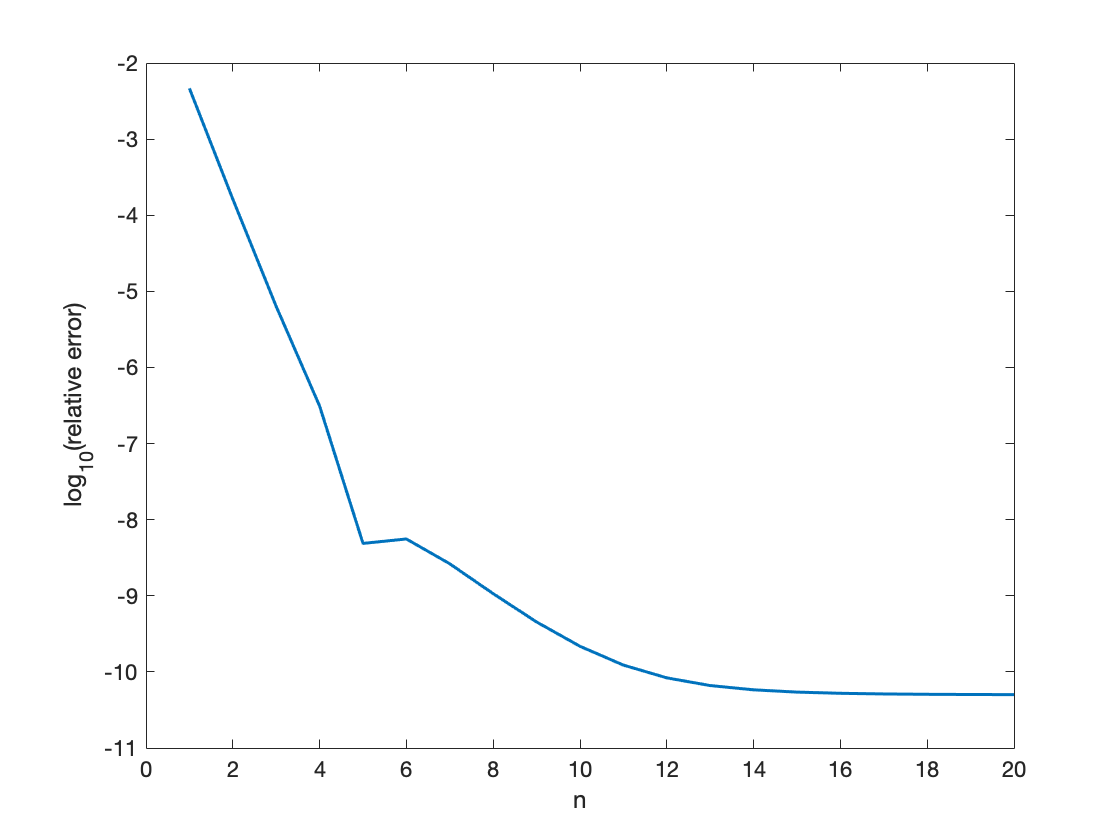
\includegraphics[width = 0.55\textwidth]{img/gauss.png} 
			\caption{相对误差与 $n$ 之间的关系}
			\label{gauss} 
		\end{figure}
		
	\end{subsection}
	
	\begin{subsection}{Romberg 求积方法的更多结果}
		
		选取不同的 $\varepsilon$,计算得相对误差的对数与 $\varepsilon$ 的关系如图 \ref{romberg} 所示。
		
		\begin{figure}[H]
			\centering
			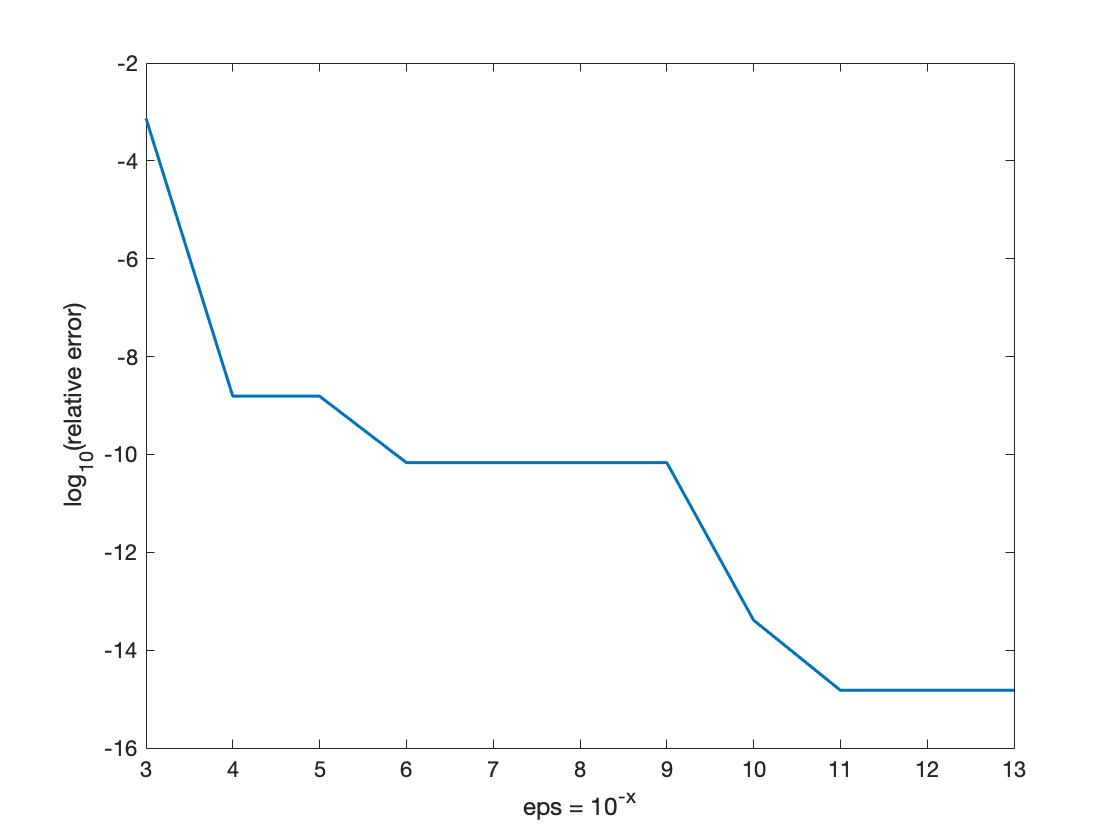
\includegraphics[width = 0.55\textwidth]{img/romberg.png} 
			\caption{相对误差与 $\varepsilon$ 之间的关系}
			\label{romberg} 
		\end{figure}
		
		从以上结果中可以看出,五点 Gauss-Legendre 复合求积公式和 Romberg 求积方法都有着良好的数值稳定性,随着 $n$ 的增加或 $\varepsilon$ 的减小,数值积分的结果都收敛至准确解。两者结果的精度优劣与选取的 $n$ 和 $\varepsilon$ 有关。
		
	\end{subsection}
	
\end{section}
	
\begin{section}{总结}
	
	本次实验对于五点 Gauss-Legendre 求积公式的复合求积公式和Romberg 求积方法进行了理论分析和编程计算,算得了 $I(f)$ 的数值解。
	
	本次实验还探究了五点 Gauss-Legendre 复合求积公式和 Romberg 求积方法的结果分别与选取的参数 $n$ 和 $\varepsilon$ 的关系。结果符合预期,适当选择参数,数值积分结果将收敛于准确解。
	
\end{section}

\end{multicols}

%\bibliographystyle{unsrt}
%\bibliography{ref.bib}

%\begin{thebibliography}{99}    %参考文献开始
%	\bibitem{ml}周志华. 机器学习[M]. 清华大学出版社, 2016.   
%\end{thebibliography}	

\end{document}

